\documentclass[11pt]{article}
\usepackage[margin=1in]{geometry}
\usepackage{booktabs}
\usepackage{graphicx}
\usepackage{microtype}
\usepackage[hidelinks]{hyperref}

\newcommand{\figN}{12.88}
\newcommand{\figFaith}{0.91}
\newcommand{\figWords}{4143}
\newcommand{\offWords}{3216}


\title{\vspace{-2em}\textbf{Vision figures --- enrichment, not a text lever}}
\author{arxivkg · generation · vision figures}
\date{}

\begin{document}
\maketitle
\vspace{-2em}

\section*{What we did}
Toggle the figure gallery on/off over the 27-topic battery. With it on, a Gemma-4-26B-Vision pass
selects architecture diagrams / result plots from the landmark papers and writes captions; each figure
is checked by a caption-faithfulness tripwire (does the caption match the image?). Scored on the text
metric vector $+$ 4-axis judge, plus the gallery's own caption-faithfulness.

\section*{Results (mean over 27 topics)}
\begin{center}\begin{tabular}{lrrrrrrr}
\toprule
figures & n figures & fig checked & caption faithfulness & words & grounded & gold recall & j coverage \\
\midrule
figures-on & 12.88 & 12.88 & 0.91 & 4143.38 & 47.88 & 0.85 & 4.75 \\
figures-off & 0.0 & 0.0 & 0.0 & 3216.12 & 47.75 & 0.92 & 4.62 \\
\bottomrule
\end{tabular}
\end{center}
\begin{center}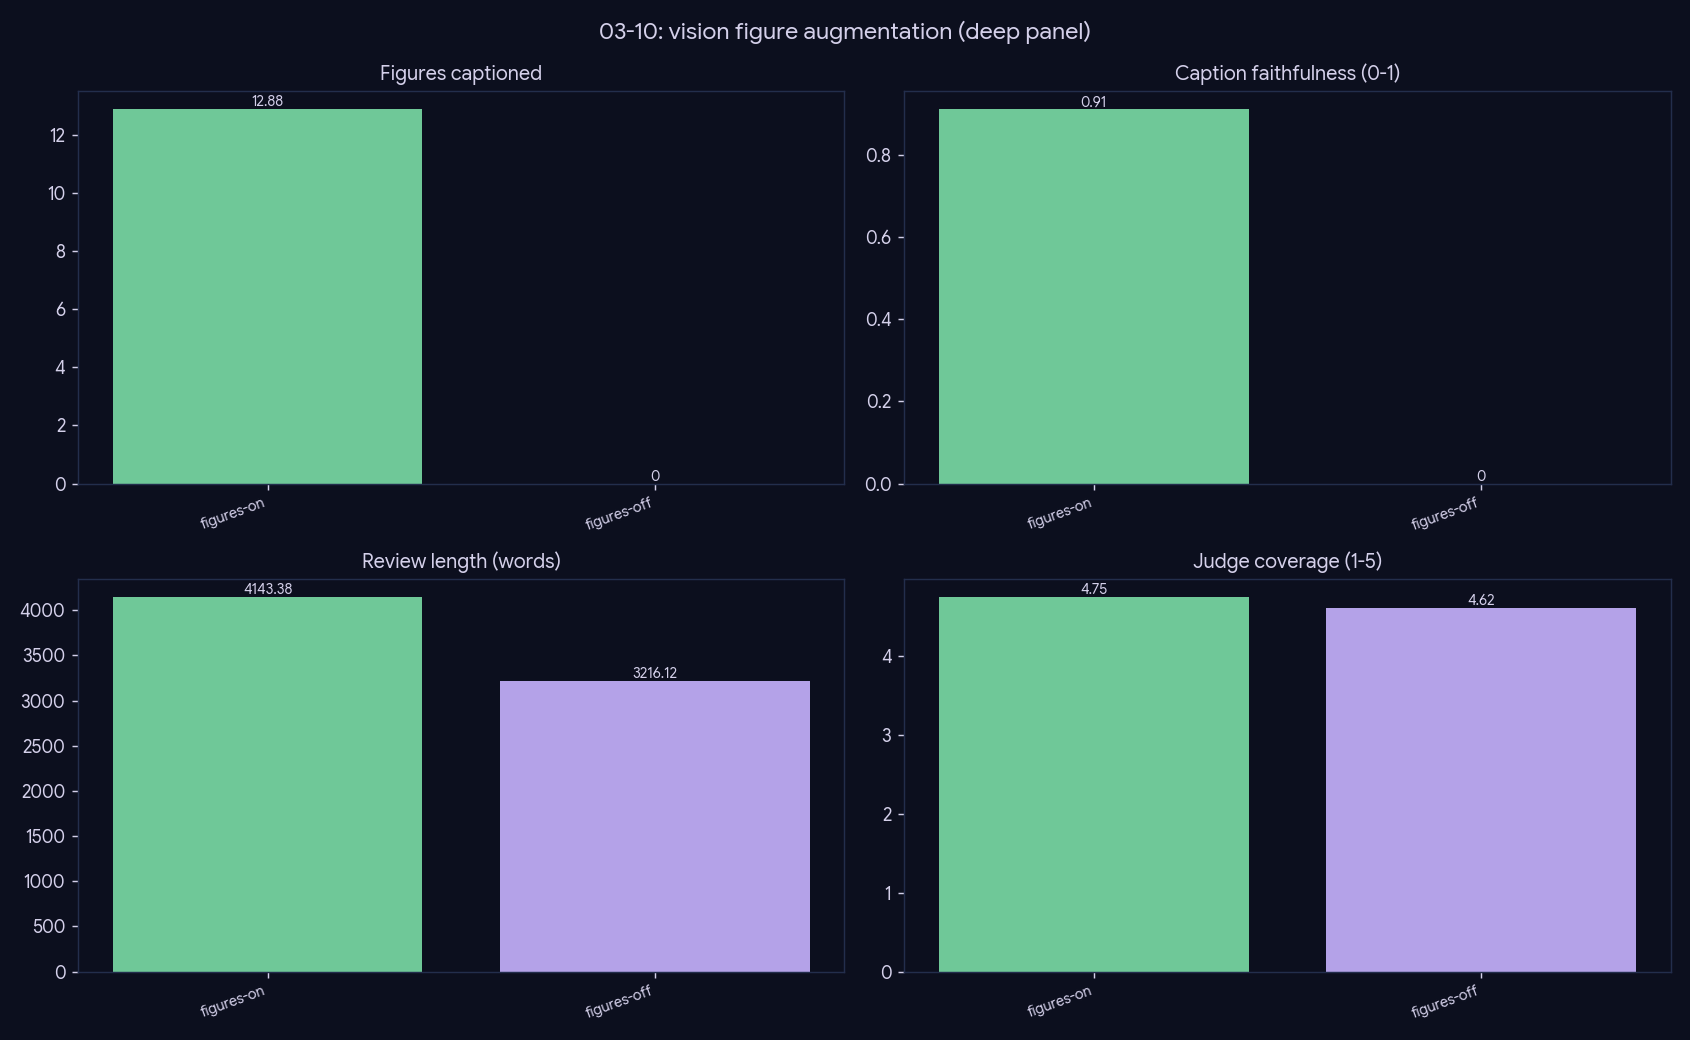
\includegraphics[width=0.95\textwidth]{../results/ablation.png}\end{center}

\section*{Conclusion}
\textbf{The figure gallery is an enrichment feature, not a lever on the text.} With it on, each review
carries \figN{} figures at \figFaith{} caption-faithfulness and grows by $\sim$1000 words
($\offWords\rightarrow\figWords$), but the 4-axis \emph{textual} judge is unchanged (coverage 4.67 vs
4.65, grounding flat) --- as expected, since the judge reads text, not images. The figures' value lives
in their \emph{own} metric (caption-faithfulness $\figFaith{}$), i.e.\ verified visual grounding the
text judge structurally cannot see. \textbf{Ship it as an option}: it makes the review materially
richer (diagrams + plots a reader wants) at the cost of $\sim$1000 words and a vision pass, without
touching textual quality --- a clean additive feature, neither a quality win nor a regression on the
text axes. \textbf{Caveat:} the only quality guarantee here is caption-faithfulness; an unfaithful
caption is the failure mode the tripwire exists to catch (\figFaith{} pass rate).

\end{document}
